\documentclass[10pt,a4paper]{article}

\usepackage[utf8]{inputenc}
\usepackage[T1]{fontenc}
\usepackage{lmodern}
\usepackage{graphicx}
\usepackage{booktabs}
\usepackage{array}
\usepackage[margin=2cm]{geometry}
\usepackage[hidelinks]{hyperref}
\usepackage{caption}
\captionsetup{font=small,labelfont=bf,skip=4pt}

\graphicspath{{./figures/}}

\newcommand{\etal}{\textit{et al.}}

\title{\bfseries Supplementary Material\\[0.2em]
\large Improving HTR Attention Maps with Register Tokens}
\author{Monika Radhakisan Chavan}
\date{}

\begin{document}
\maketitle
\vspace{-2.5em}

\noindent This document collects the per-group training curves referenced in Section~5 of the main report and expands the four future-work extensions listed in Section~7.

\section*{S1.~Per-Group Training Curves}

Figure~\ref{fig:supp_curves} shows the per-group CER convergence for the four experiment blocks not shown in the main report (architecture ablations, pretrained-lane fine-tuning, READ2016 register sweep, synthetic pretraining). The two catastrophically-failing rows of the architecture ablation (no CNN stem, legacy row-major layout) sit as flat lines near $73\%$ from epoch~$1$ and are visible at the top of the top-left panel. The naive-uniform-LR ViT-B/16 fine-tune stays above $70\%$ throughout the pretrained panel, in contrast to the two-group-LR and LLRD runs that converge cleanly. The READ2016 register variants collapse onto essentially the same trajectory, mirroring the IAM behaviour in the main report. The synthetic-pretraining curves terminate at the cluster walltime rather than at their intended epoch budget; the reported numbers are lower bounds on convergence.

\begin{figure}[h]
\centering
\begin{minipage}{0.48\linewidth}\centering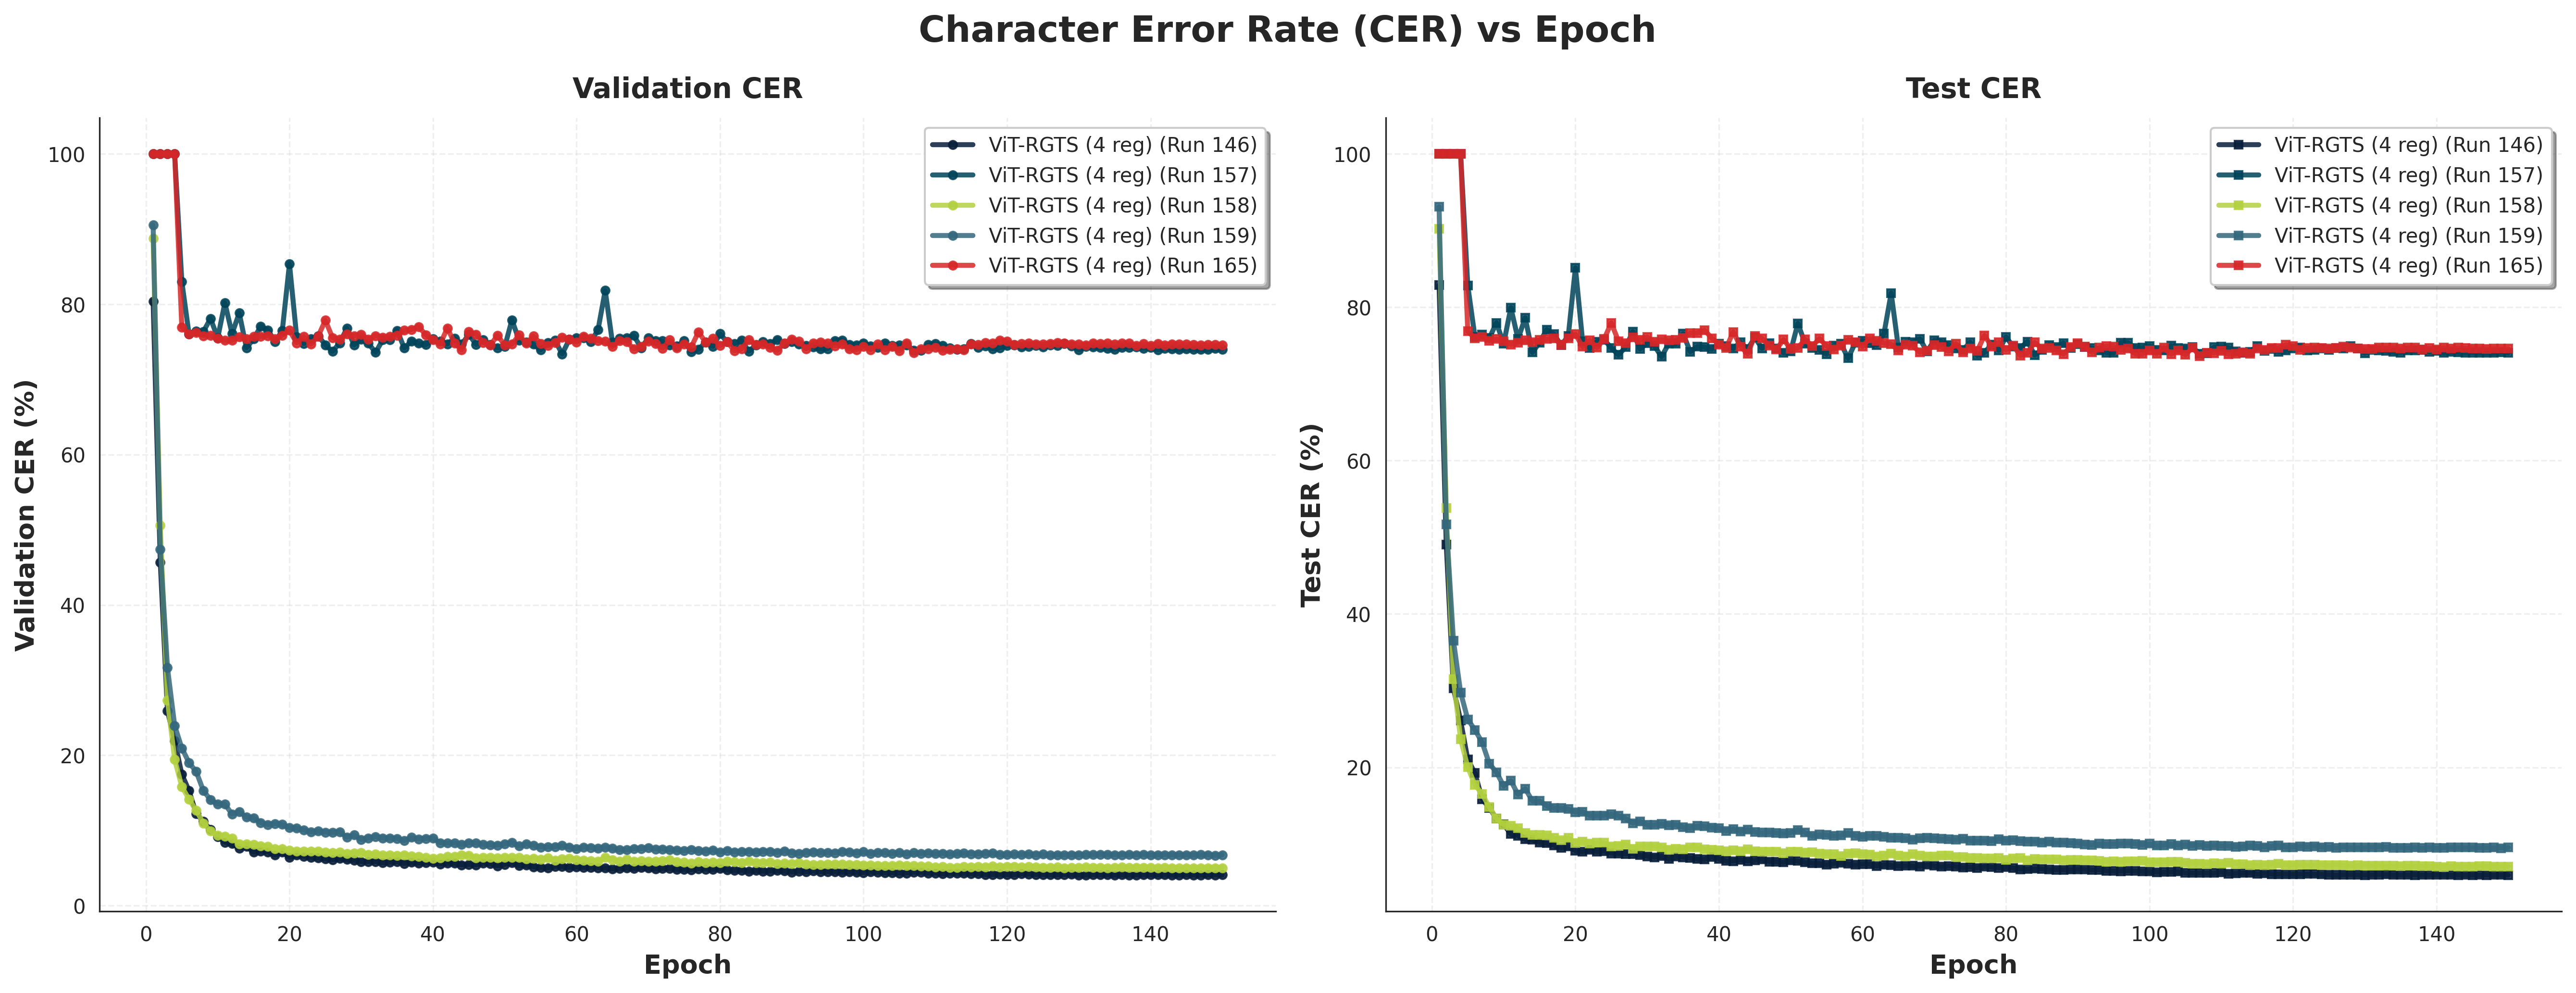
\includegraphics[width=\linewidth]{supp_training_curves_ablations_cer}\\{\footnotesize (a) Architecture ablations}\end{minipage}\hfill
\begin{minipage}{0.48\linewidth}\centering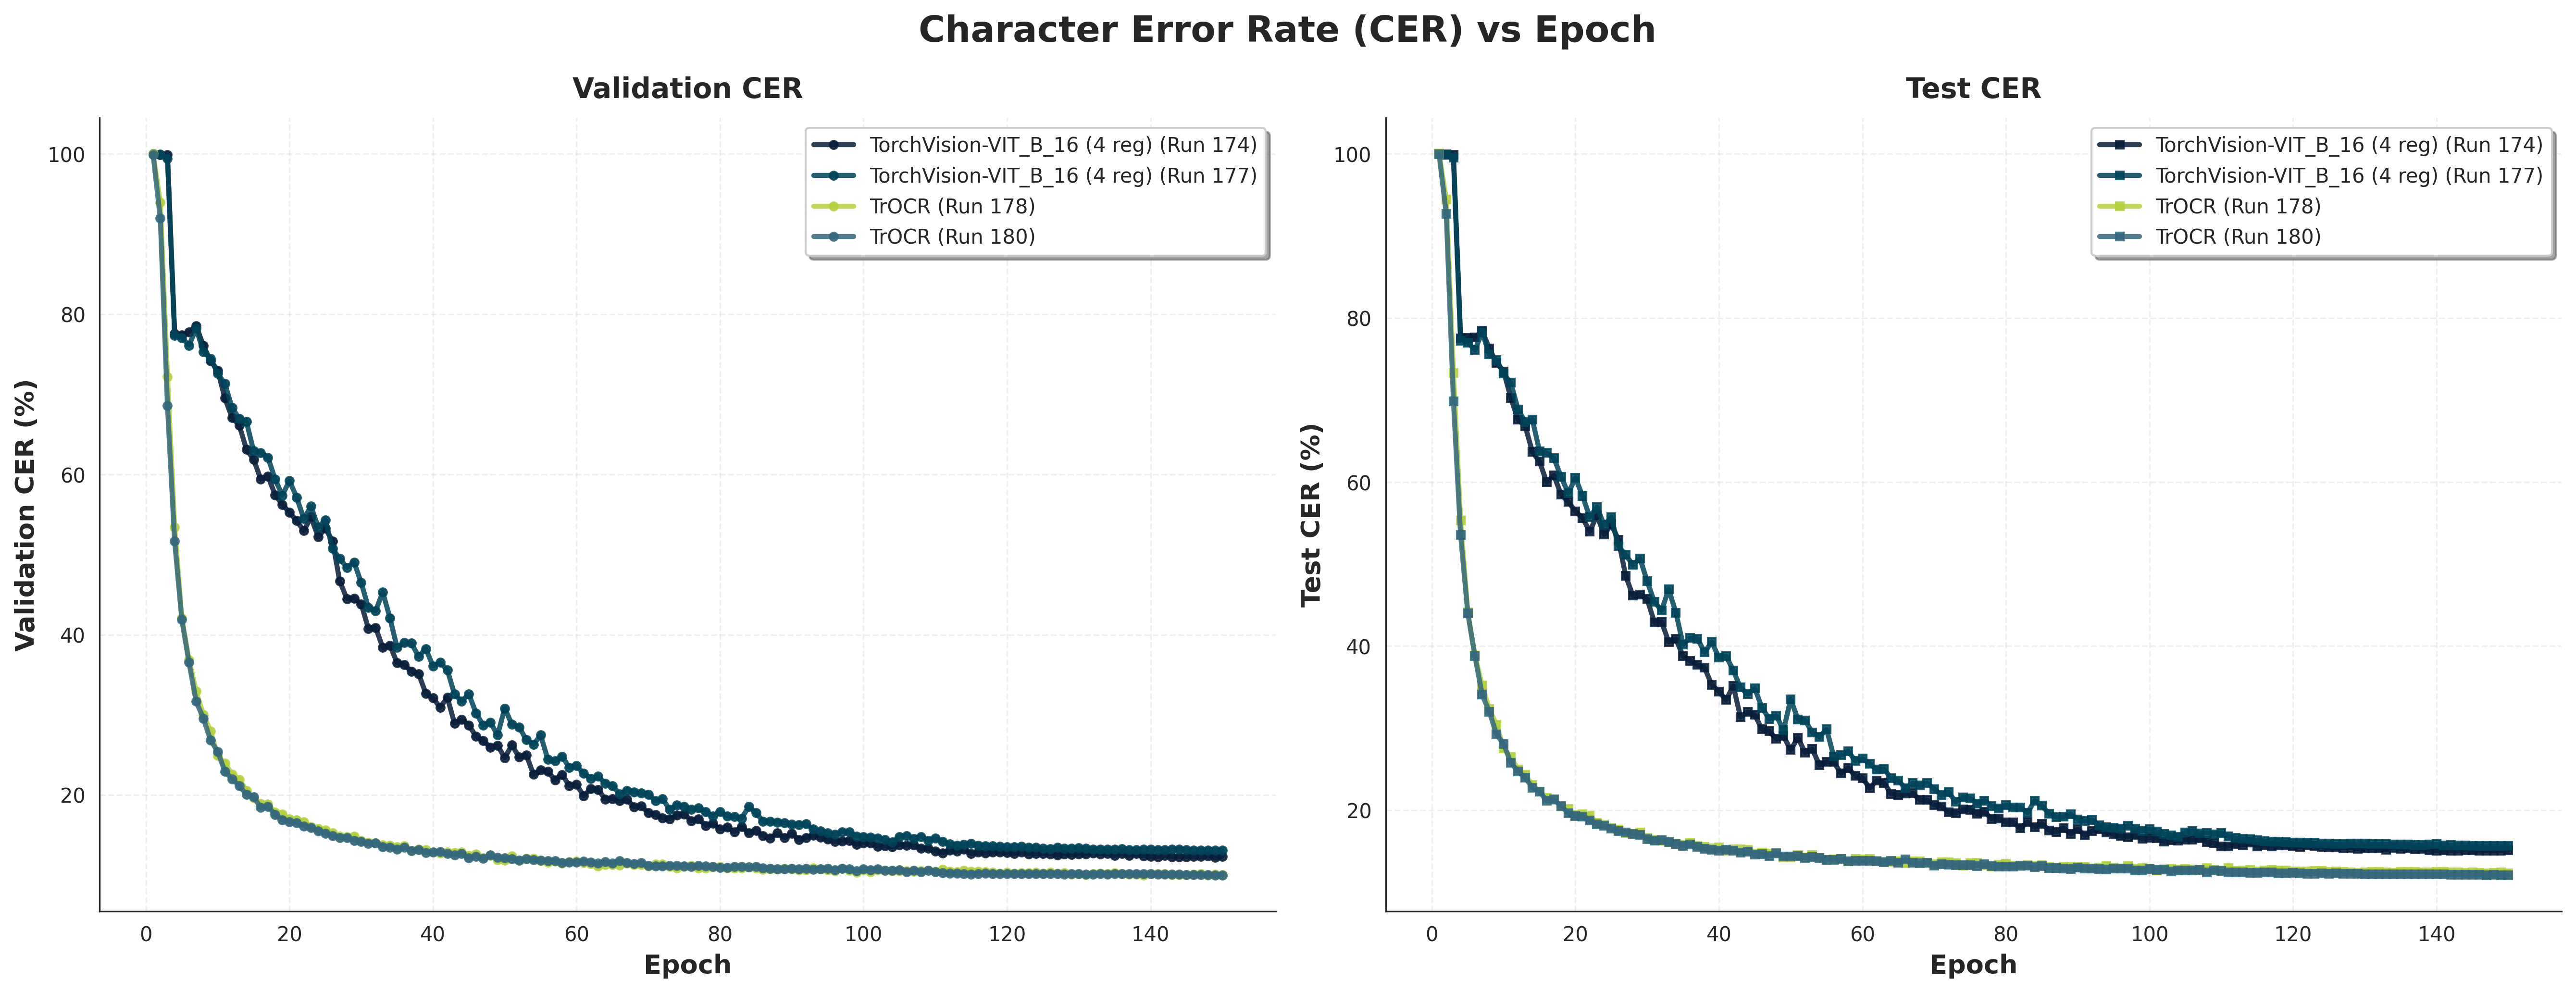
\includegraphics[width=\linewidth]{supp_training_curves_pretrained_cer}\\{\footnotesize (b) Pretrained-lane fine-tuning}\end{minipage}\\[0.4em]
\begin{minipage}{0.48\linewidth}\centering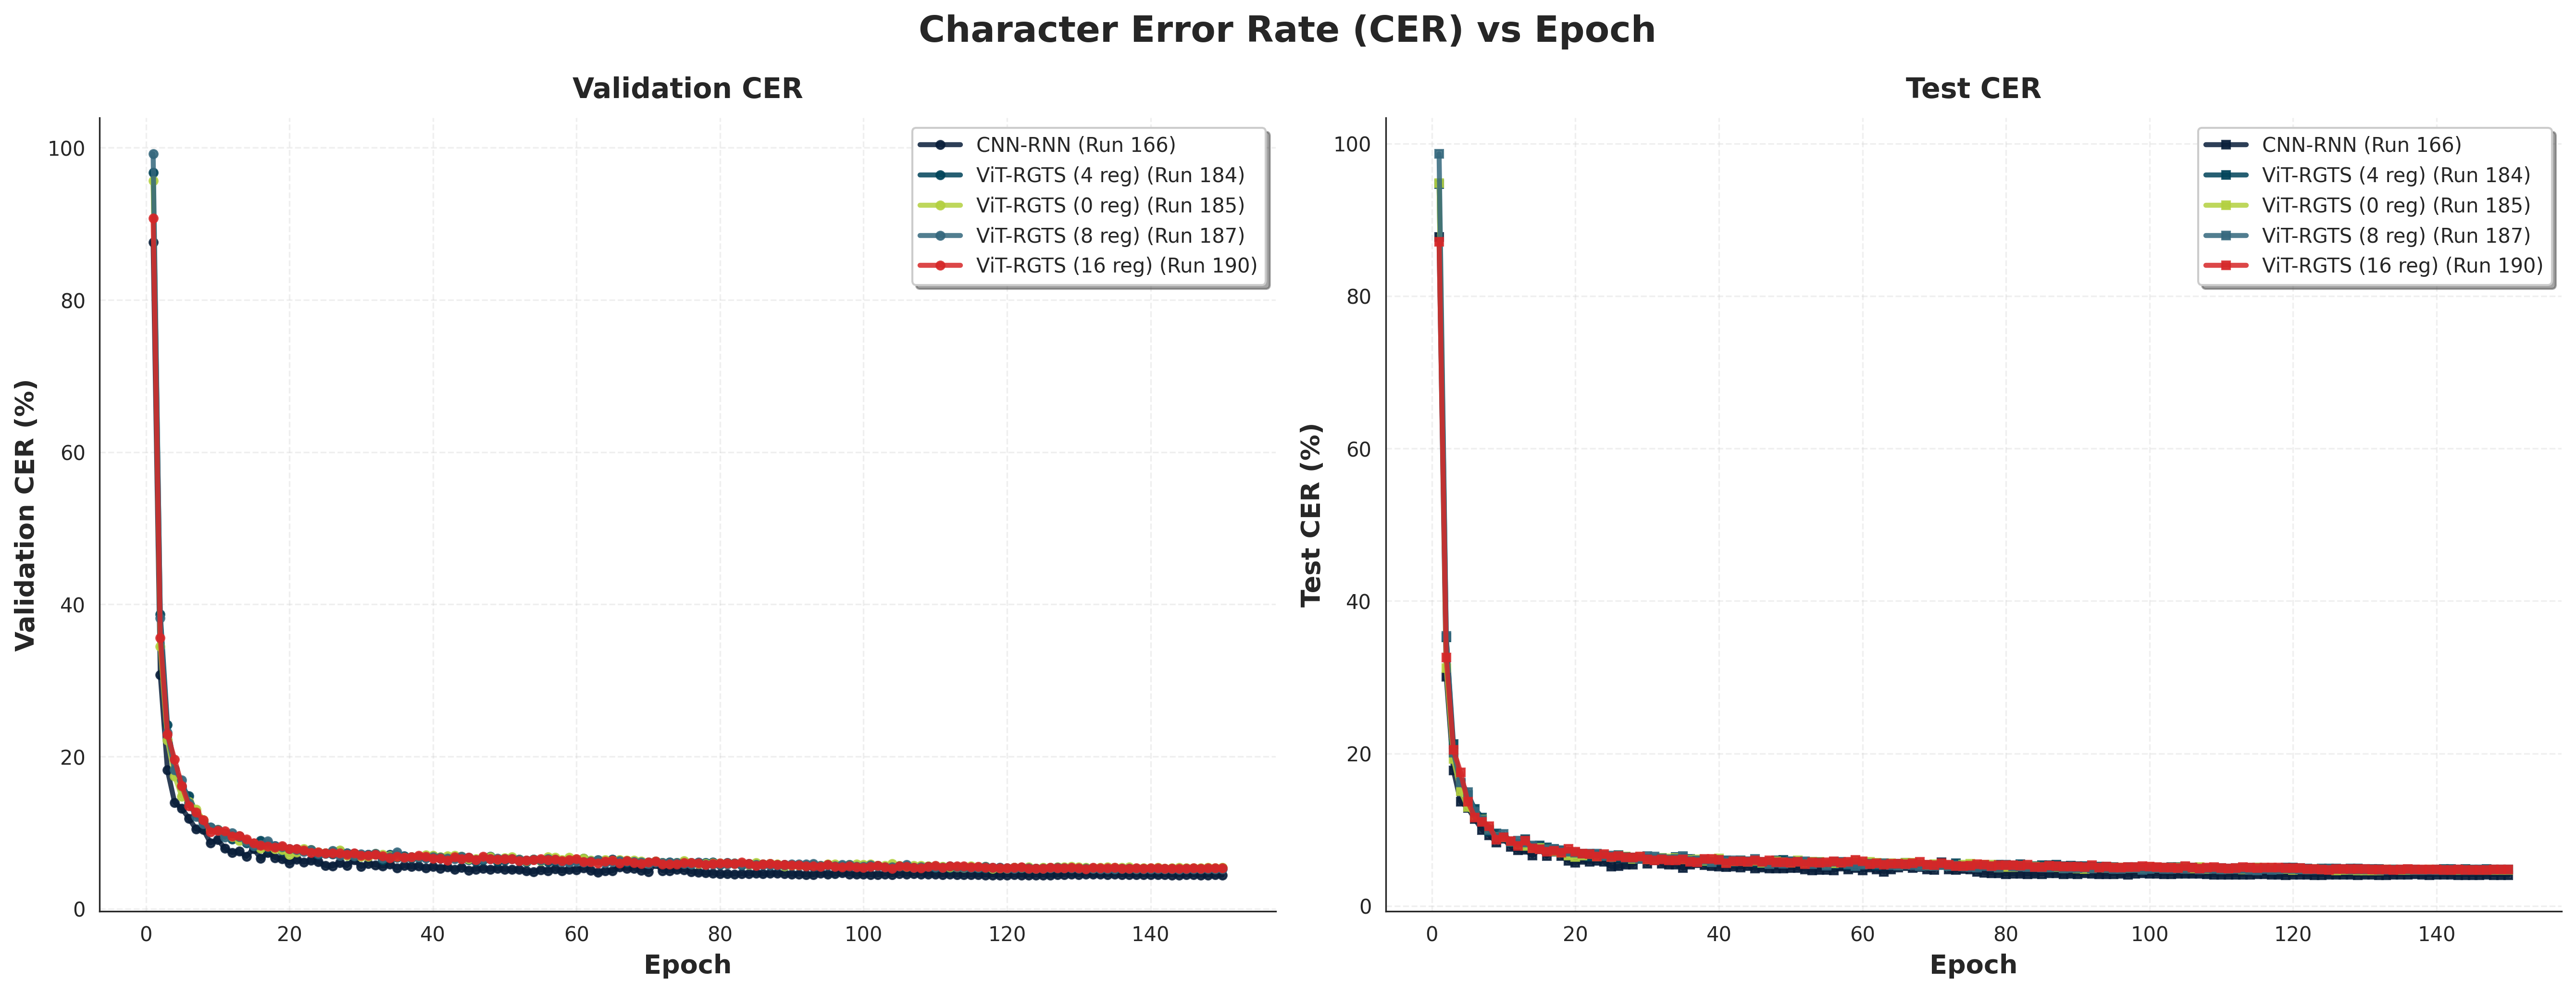
\includegraphics[width=\linewidth]{supp_training_curves_read2016_cer}\\{\footnotesize (c) READ2016 register sweep}\end{minipage}\hfill
\begin{minipage}{0.48\linewidth}\centering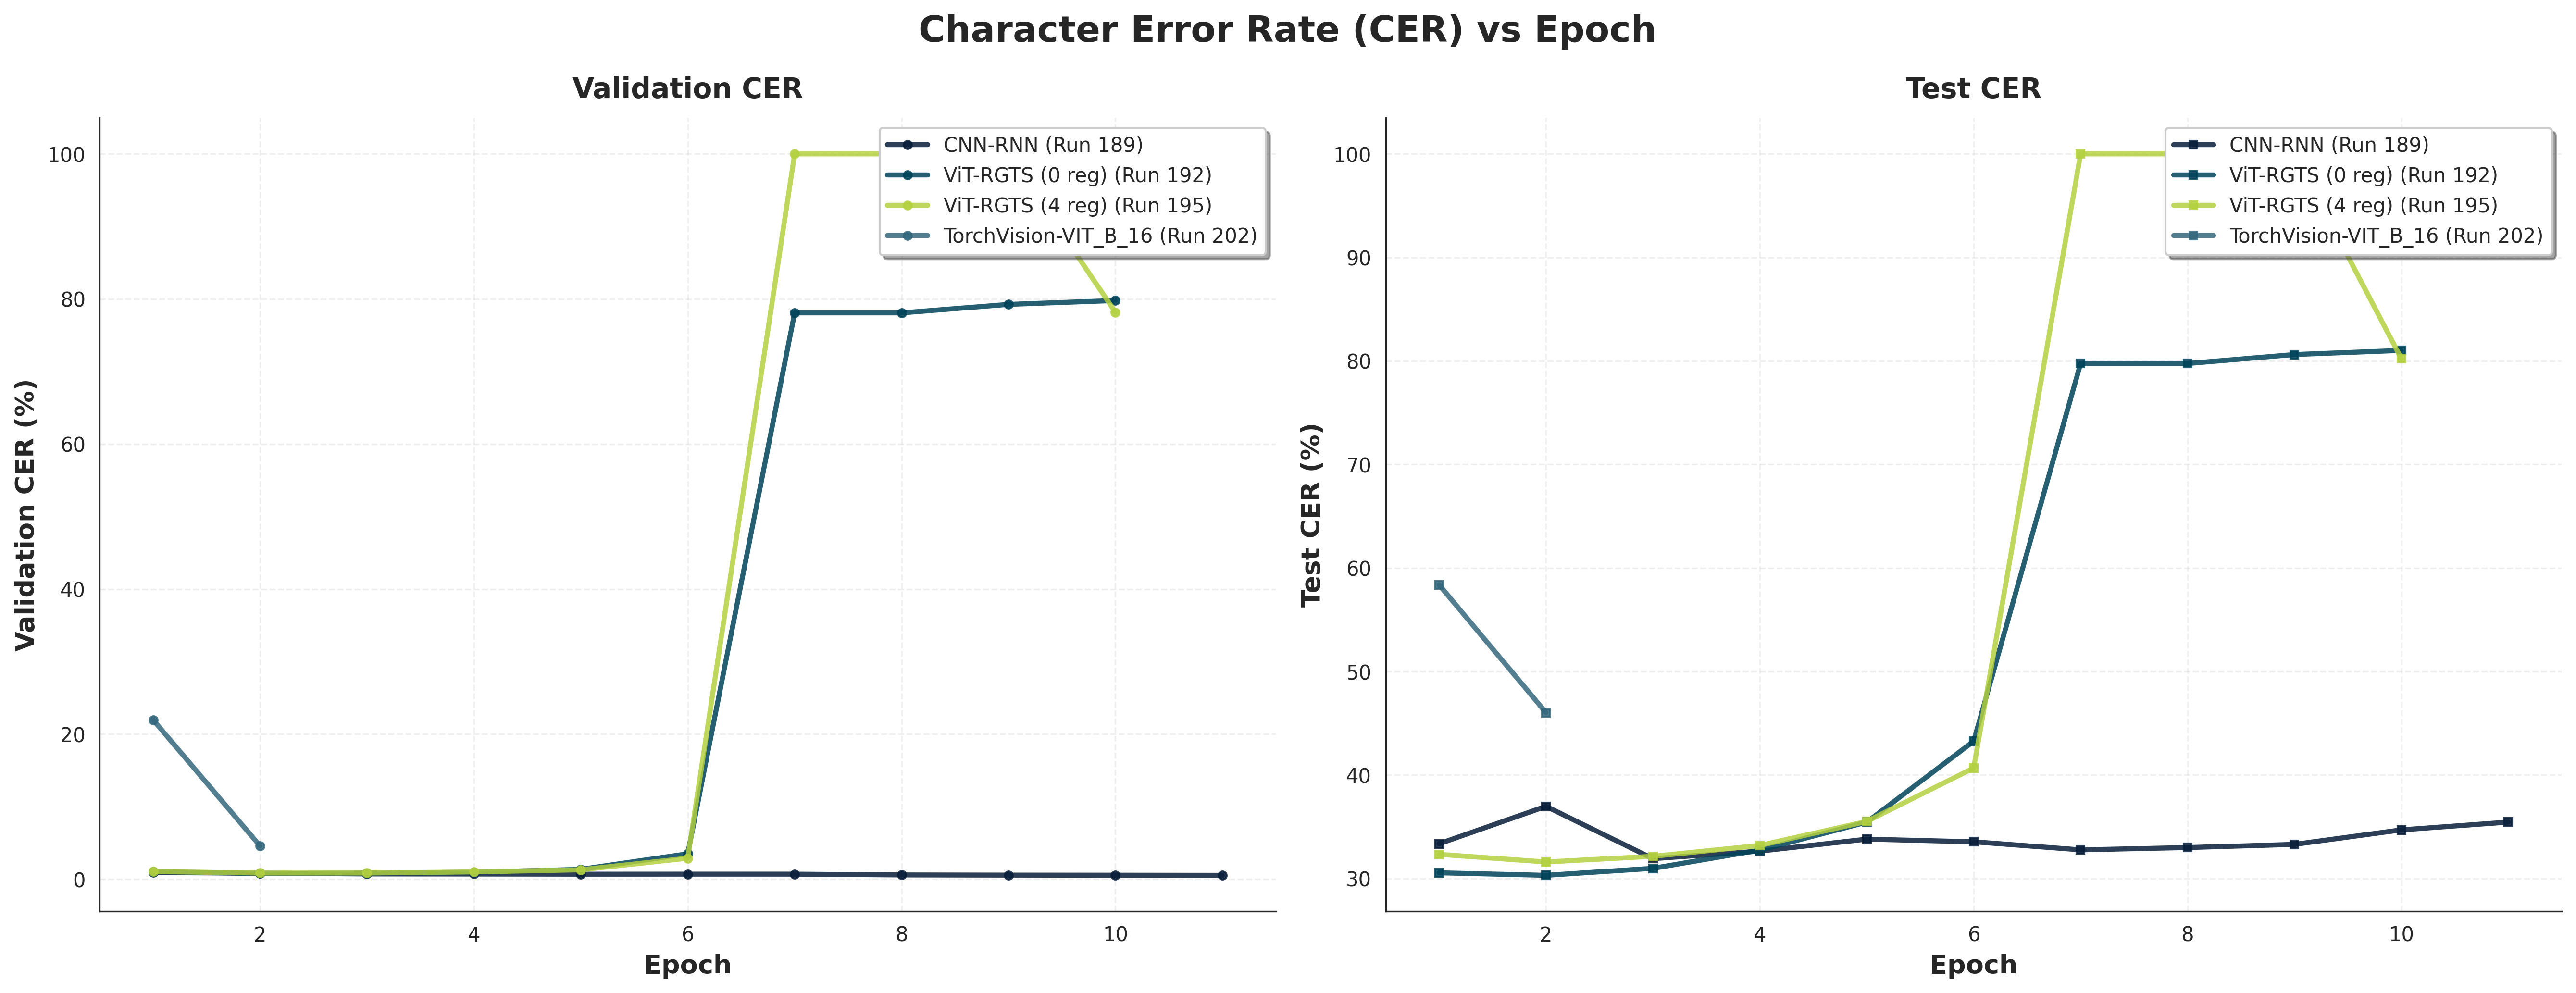
\includegraphics[width=\linewidth]{supp_training_curves_synthetic_cer}\\{\footnotesize (d) Synthetic pretraining (walltime-truncated)}\end{minipage}
\caption{Test-CER convergence for the four experiment blocks not shown in the main report.}
\label{fig:supp_curves}
\end{figure}

\section*{S2.~Extension Proposals}

\paragraph{Writer identification via VLAC over ViT-RGTS attention.} The Souibgui~\etal~\cite{souibgui2022vlac} VLAC construction can be plugged in directly on top of the ViT-RGTS attention output. At inference, for every recognized character in every training-set page, extract the CTC peak column $t_c$, the patch-token embedding at $t_c$ from the final Transformer layer, and the attention weight vector at the character's query. Cluster the patch-token embeddings across the training corpus into $K$ character-prototype centroids, assign each character to its nearest prototype, and accumulate residual VLAC-style aggregates per prototype into a per-page descriptor. Evaluate with writer-retrieval mAP, top-1, and top-5 on IAM writer-ID splits. This is the single most direct test of whether the interpretability claim in Section~5.3 of the main report translates into a downstream task.

\paragraph{CLS-augmented CTC ViT.} The residual sink pattern documented in Section~5.3 of the main report is attributed to the absence of a CLS-style aggregate query. Adding a single CLS token in front of the register block, supervised at training time by a light auxiliary loss (for example a line-level writer classification head that is unrelated to the CTC objective), should let the registers take over the global-information role more completely. The predicted signature is a flip of the token-norm asymmetry: registers now carrying more L2 norm than patches, matching the classification-ViT direction Darcet~\etal~\cite{darcet2024registers} report.

\paragraph{Attention-entropy regularizer.} A low-weight entropy regularizer on the final-layer patch attention would provide the gradient signal that CTC lacks. Given the set $\mathcal{T}$ of non-blank CTC query positions and Shannon entropy $H$, the auxiliary loss is $\mathcal{L}_{\mathrm{aux}} = \beta \cdot |\mathcal{T}|^{-1} \sum_{t \in \mathcal{T}} H(\mathbf{a}_t^{(L)})$, added to the primary CTC loss. A starting range for $\beta$ is $[10^{-3}, 10^{-2}]$; larger values flatten attention rather than sharpen it. The regularizer should be evaluated jointly against CER and against the attention-concentration metrics of Section~4.3, not against CER alone.

\paragraph{Synthetic-to-IAM curriculum.} The synthetic-pretraining lane was walltime-truncated. A converged run --- pretrain to convergence on the ${\sim}950$K synthetic corpus, then fine-tune on IAM with a decayed learning rate --- would test whether the CER gap between ViT-RGTS and the CNN--RNN baseline closes under pretraining, without altering the register-attention story.

\bibliographystyle{plain}
\bibliography{references}

\end{document}
